
\documentclass{book}
\usepackage[utf8]{inputenc}
\usepackage{graphicx}
\usepackage{tikz}
\usepackage{float}
\usepackage{wrapfig,lipsum}
\usepackage{svg}
\usepackage{mathtools}
\usepackage{tabu}
\usepackage{subcaption}
\usepackage[a4paper, total={6in, 8in}]{geometry}

\definecolor{bg}{rgb}{0.95,0.95,0.95}




\begin{document}


\newcommand{\vecthreeBF}[1]{\vec{\textbf{#1}}}
\newcommand{\vecthree}[1]{\vec{#1}}
\newcommand{\vecNum}[3]{(#1, #2, #3)}

\newcommand{\parDeriv}[2]{\frac{\partial #1}{\partial #2}}
\newcommand{\parDerivS}[2]{\frac{\partial^2 #1}{\partial #2^2}}
\newcommand{\derivS}[2]{\frac{d^2 #1}{d#2^2}}

\newcommand{\dotProdBF}[2]{\vecthreeBF{#1} \cdot \vecthreeBF{#2}}
\newcommand{\dotProd}[2]{\vecthree{#1} \cdot \vecthree{#2}}

\newcommand{\crossProdBF}[2]{\vecthreeBF{#1} \times \vecthreeBF{#2}}
\newcommand{\crossProd}[2]{\vecthree{#1} \times \vecthree{#2}}

\newcommand{\e}{$\textbf{e}^-$ }
\newcommand{\egun}{$\textbf{e}^-$-gun }
\newcommand{\eB}{$\textbf{e}^-$ - $\vecthreeBF{B}$ }
\newcommand{\eE}{$\textbf{e}^-$ - $\vecthreeBF{E}$ }
\newcommand{\eEM}{$\textbf{e}^-$ - \textbf{EM} }
\newcommand{\ee}{$\textbf{e}^-$ - $\textbf{e}^-$ }


\newcommand{\fromeq}[1]{\textit{equation \ref{eq:#1}}}
\newcommand{\fromeqs}[2]{\textit{equations \ref{eq:#1} and \ref{eq:#2}}}
\newcommand{\fromeqsth}[3]{\textit{equations \ref{eq:#1}, \ref{eq:#2} and \ref{eq:#3}}}
\newcommand{\fromeqsf}[4]{\textit{equations \ref{eq:#1}, \ref{eq:#2}, \ref{eq:#3} and \ref{eq:#4}}}

\newcommand{\fromfig}[1]{\textit{figure \ref{fig:#1}}}
\newcommand{\fromfigs}[2]{\textit{figures \ref{fig:#1} and \ref{fig:#2}}}
\newcommand{\fromfigf}[4]{\textit{figures \ref{fig:#1}, \ref{fig:#2}, \ref{fig:#3} and \ref{fig:#4}}}

\newcommand{\fromsec}[1]{\textit{section \ref{sec:#1}}}
\newcommand{\fromsecs}[2]{\textit{sections \ref{sec:#1} and \ref{sec:#2}}}

\newcommand{\fromapp}[1]{\textit{Appendix \ref{appendix:#1}}}

\newcommand{\fromtab}[1]{\textit{Table \ref{tab:#1}}}
\newcommand{\fromtabs}[2]{\textit{Tables \ref{tab:#1} and \ref{tab:#2}}}



%----../../..++++.

%%%%%%
% Start of techd.tex
\section{Technical Drawing}
Technical drawings of the design mentioned in \fromsec{final_design} can be found in \fromfigs{techd_rhod}{techd_mid}, \fromfig{techd_up} of \fromapp{supp}.

\vspace{-20pt}
\begin{figure}[H]
    \centering
    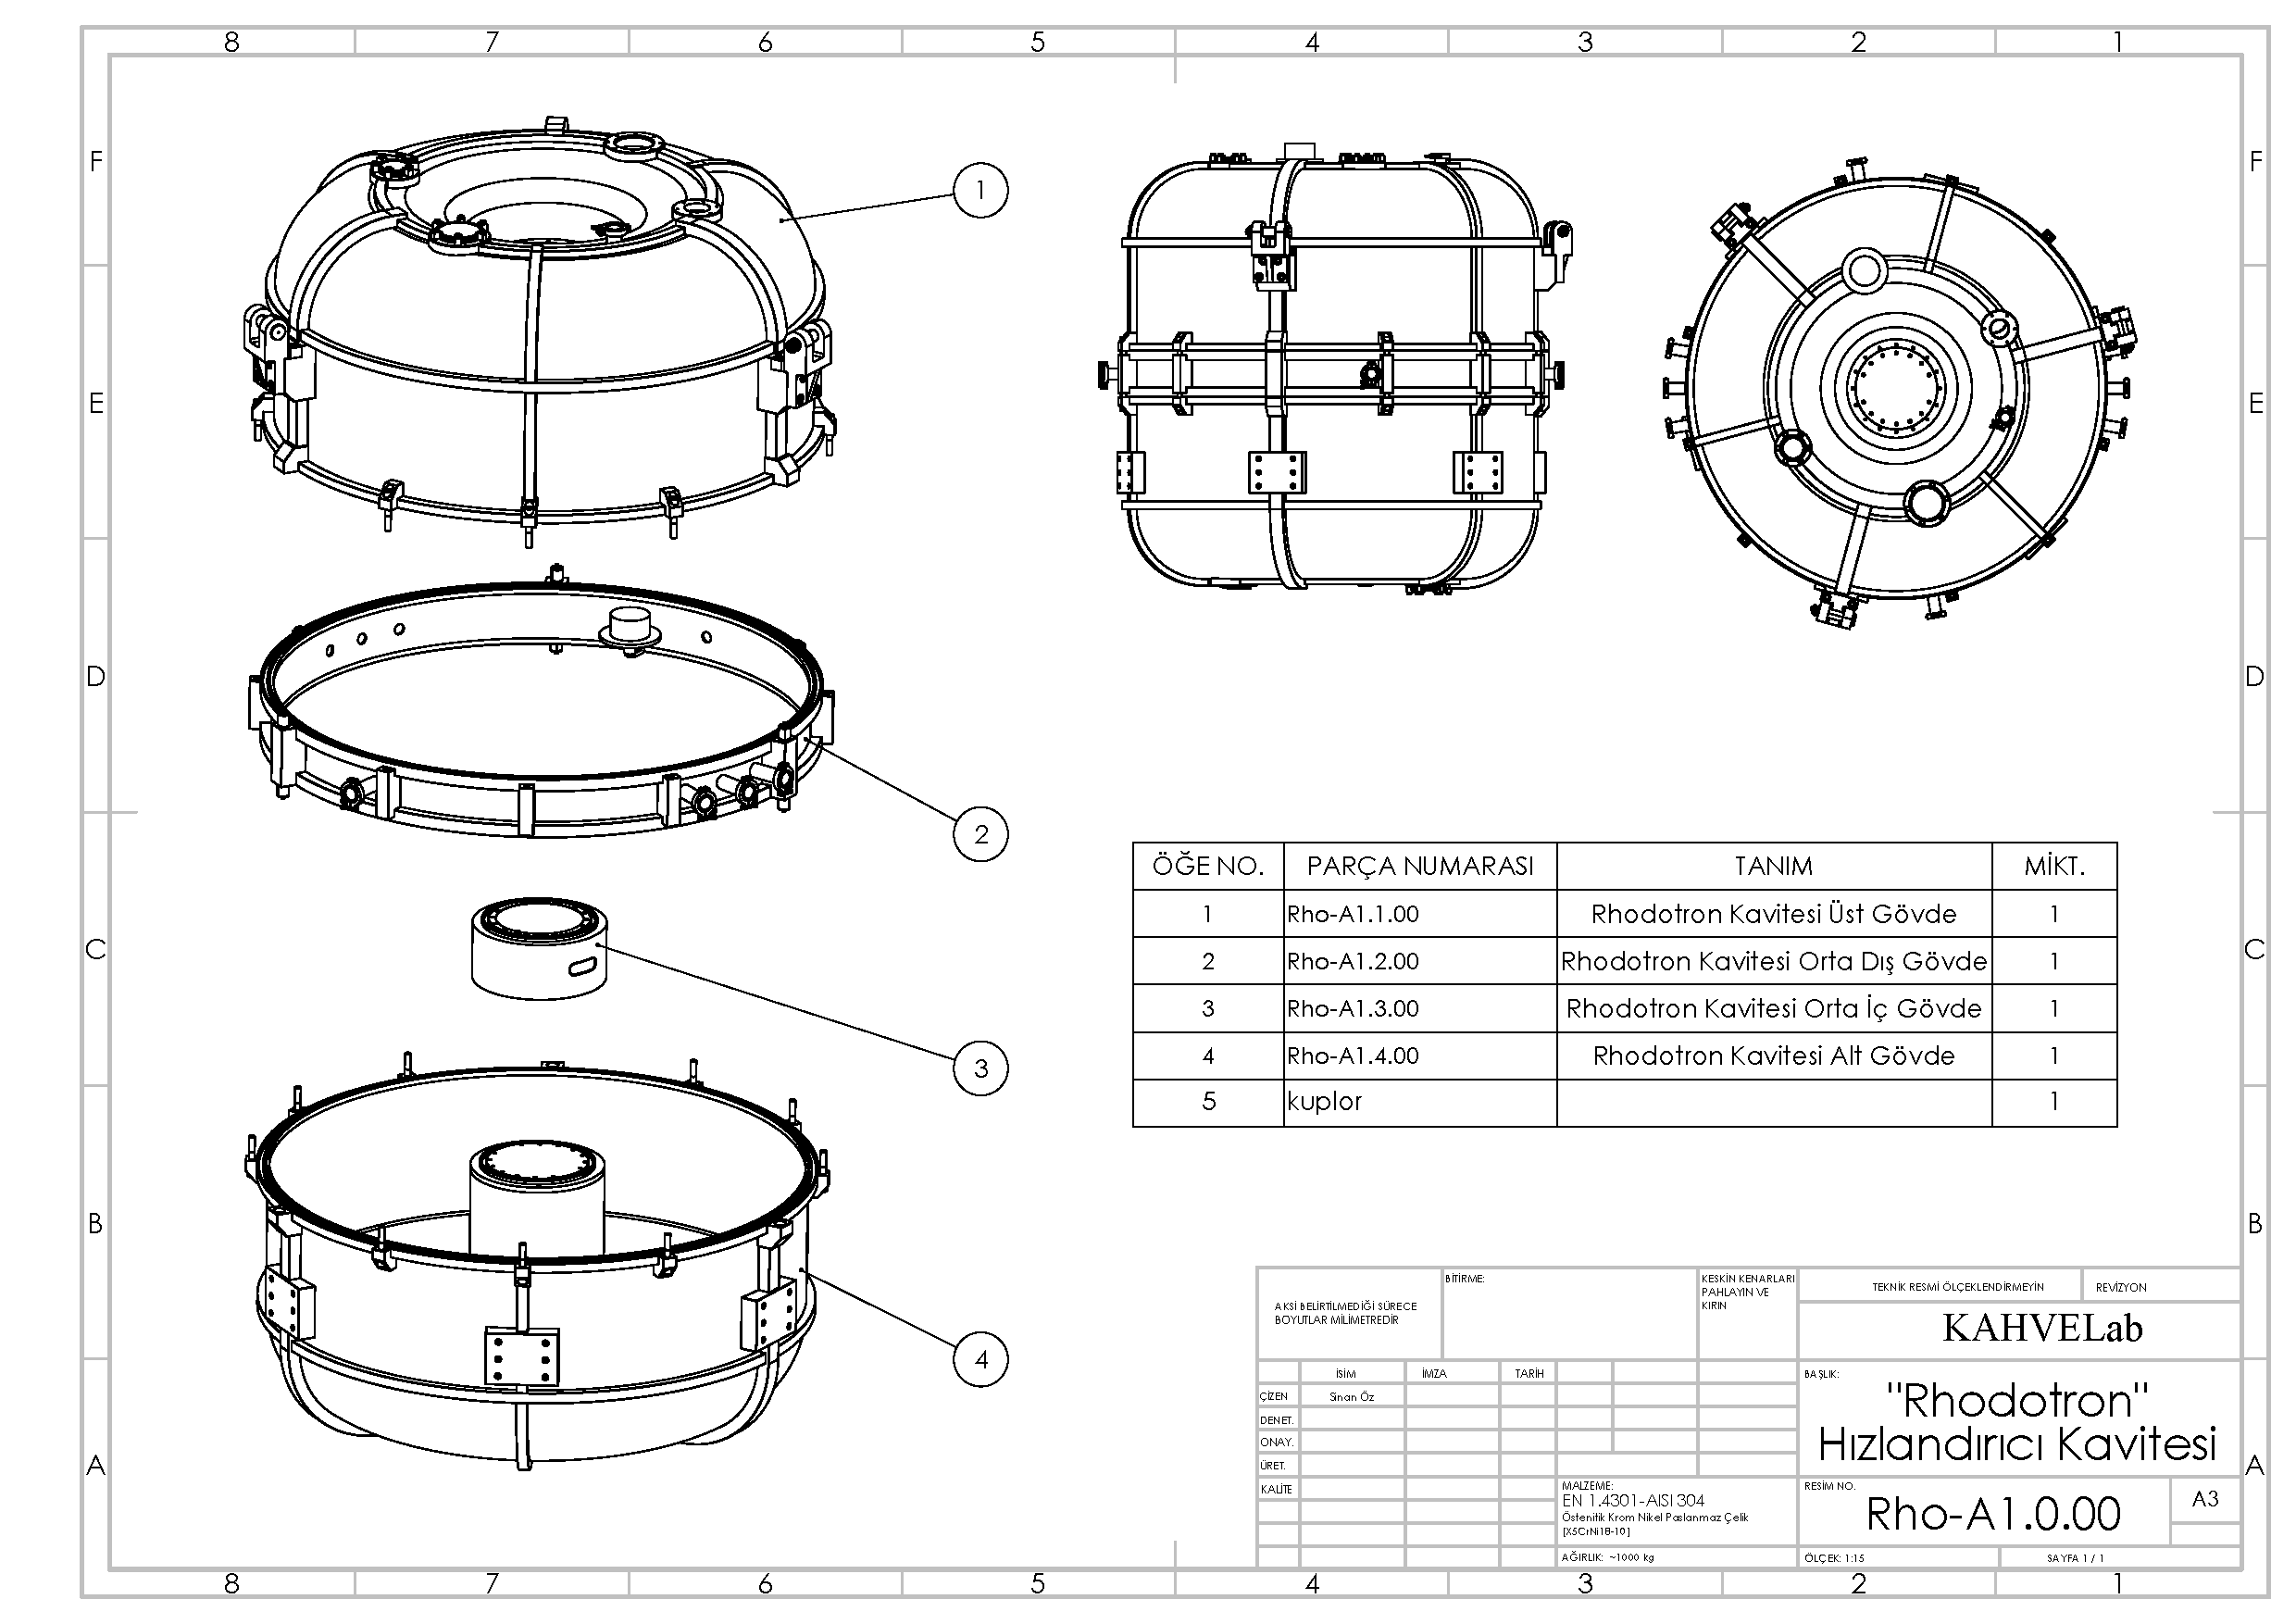
\includegraphics[angle=270,origin=c, width=.95\linewidth]{../../../figures/teknikcizim/Rho-A1.0.00.pdf}
    \vspace{5pt}
    \caption{Technical drawing of the rhodotron cavity \cite{sinan}.}
    \label{fig:techd_rhod}
\end{figure}
\clearpage
\begin{figure}[!th]
    \centering
    \includegraphics[angle=270,origin=c, width=.95\linewidth]{../../../figures/teknikcizim/Rhodotron Elektron Hizlandirici Sistemi.pdf}
    \vspace{10pt}
    \caption{Technical drawing of middle part of the cavity which contains the beam line \cite{sinan}.}
    \label{fig:techd_mid}
\end{figure}

%%%%%%

\end{document}